  \def\thelstlisting{}

%不需要区分奇偶页的请使用下面一行
\documentclass[a4paper,AutoFakeBold,oneside,12pt]{book}
%需要区分奇偶页的(即每一章第一页一定在奇数页上)请使用下面一行
%\documentclass[a4paper,AutoFakeBold,openright,12pt]{book}
\usepackage{XUPTthesisbachelor}
\usepackage{setspace}


%%%%%%%%%%%%%%%%%%%%%%%%% Begin Documents %%%%%%%%%%%%%%%%%%%%%%%%%%
\begin{document}

% 封面和前置文档
\blankmatter
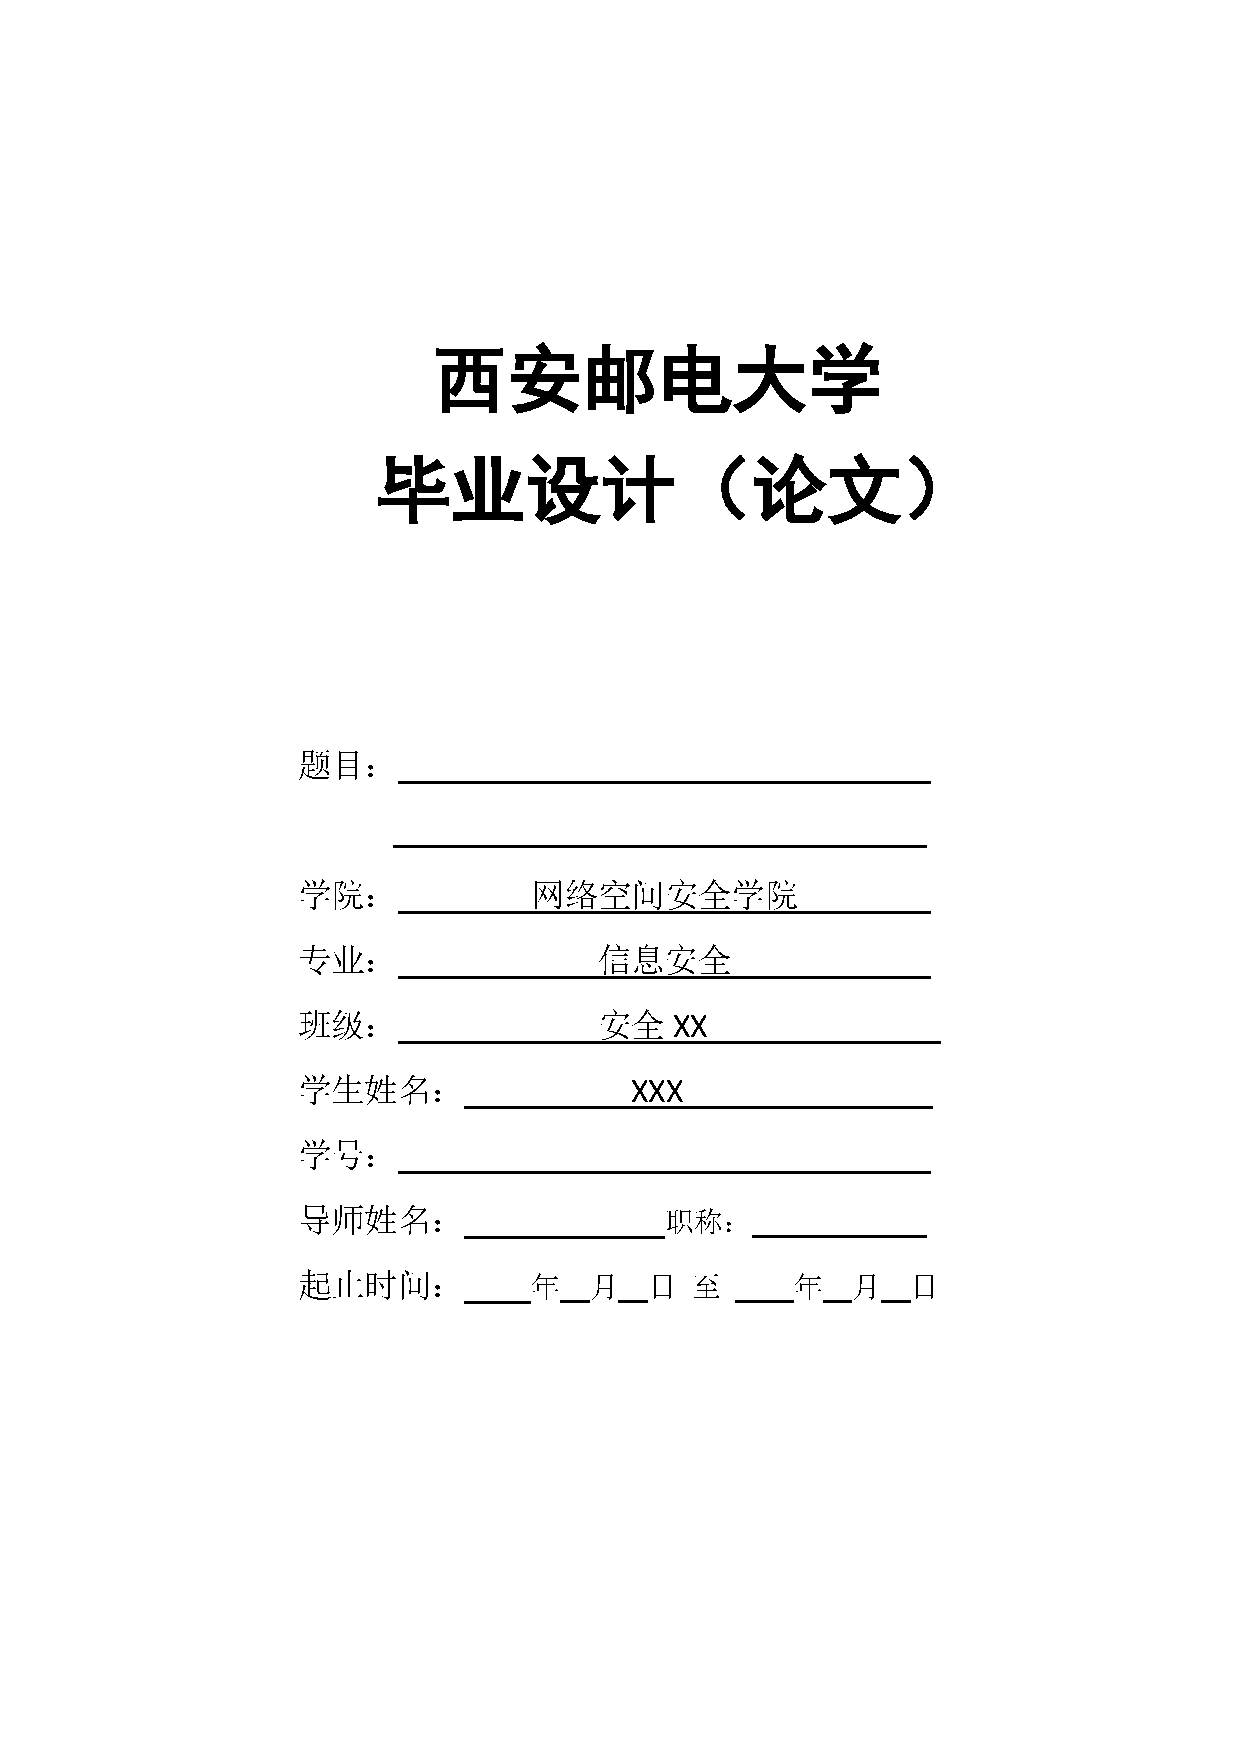
\includepdf[pages=-]{docs/cover_prevword.pdf}  


% 论文中文题目
\def\thesistitle{社猜猜看这个毕设题目是什么}

% 论文英文题目
%提示:英文摘要页的标题注意格式要求。
\def\thesistitleen{HAVE A TRY TO GUESS WHAT THE TITLE IS}

% Thank Words
\def\thankwords{
时光荏苒,四年本科生涯即将结束,回首往昔,时光留存于西邮校园的各个角落里,老师和同学们的帮助我铭记在心。我愿将一腔热情,满怀感激化作对师长、朋友的美好祝愿。

凡是过往,皆为序章。

}

    % Main items 

% 中文摘要
\def\abstractzh{
中文摘要内容。

%摘要结束
}

% 中文关键字 
% TODO: 改成可变长度的
\def\abszhkeyone{自然语言处理;}
\def\abszhkeytwo{深度学习}



% ABSTRACT
\def\abstracten{
English abstract. 

%Abstract done
}

% Key Words 
% TODO: 改成可变长度的
\def\absenkeyone{Natural language processing;}
\def\absenkeytwo{deep learning}




  % Abstract
\fancypagestyle{plain}{\pagestyle{frontmatter}}
\frontmatter\tableofcontents % Content


% 正文
\newpage\mainmatter
\fancypagestyle{plain}{\pagestyle{mainmatter}}
%\let\cleardoublepagebak=\cleardoublepage
%\let\cleardoublepage\relax % Make new chapter stay on old page

%%%%%%%%%%%%%%%%%%%%%%%%%%%%% Main Area %%%%%%%%%%%%%%%%%%%%%%%%%%

\chapter{Latex文本编辑}
\section{二级标题}
\subsection{三级标题}
\LaTeX,本模板建议使用overleaf进行在线编辑,可以尝试使用VSCode+TexLive编辑。

参考 https://zhuanlan.zhihu.com/p/43133114

在latex符号使用请自行学习并查阅相关文档。


\chapter{正文内的元素插入}
\section{公式的插入}
在行文中,使用 \$ ... \$ 可以插入行内公式。如果需要对行间公式进行编号,则可以使用 equation 环境。

使用他人文献内公式推荐使用Mathpix Snipping Tool,可以将公式自动转换为latex格式。
\begin{equation}
\begin{aligned}
f(x)=\left\{\begin{array}{ll}
+1, & x \geqslant 0 \\
-1, & x<0
\end{array}\right.
\end{aligned}
\end{equation}

\begin{equation}
\begin{aligned}
y=f(w \cdot x+b)=f\left(w_{1} x_{1}+w_{2} x_{2}+\dots+w_{n-1} x_{n-1}+w_{n} x_{n}+b\right)
\end{aligned}
\end{equation}




\section{图片的插入}
单图,如图2.1所示:
\xuptfigure[width=0.6\textwidth]{pictures/rnn}{循环神经网络}{label}

双图并列,如图2.2所示:

\begin{figure}[!htbp]
    \centering
    \subfloat[]{ %[]对齐方式,t为top,b为bottom,留空即可
	\label{Fig:a1} % 子图1标签名
    	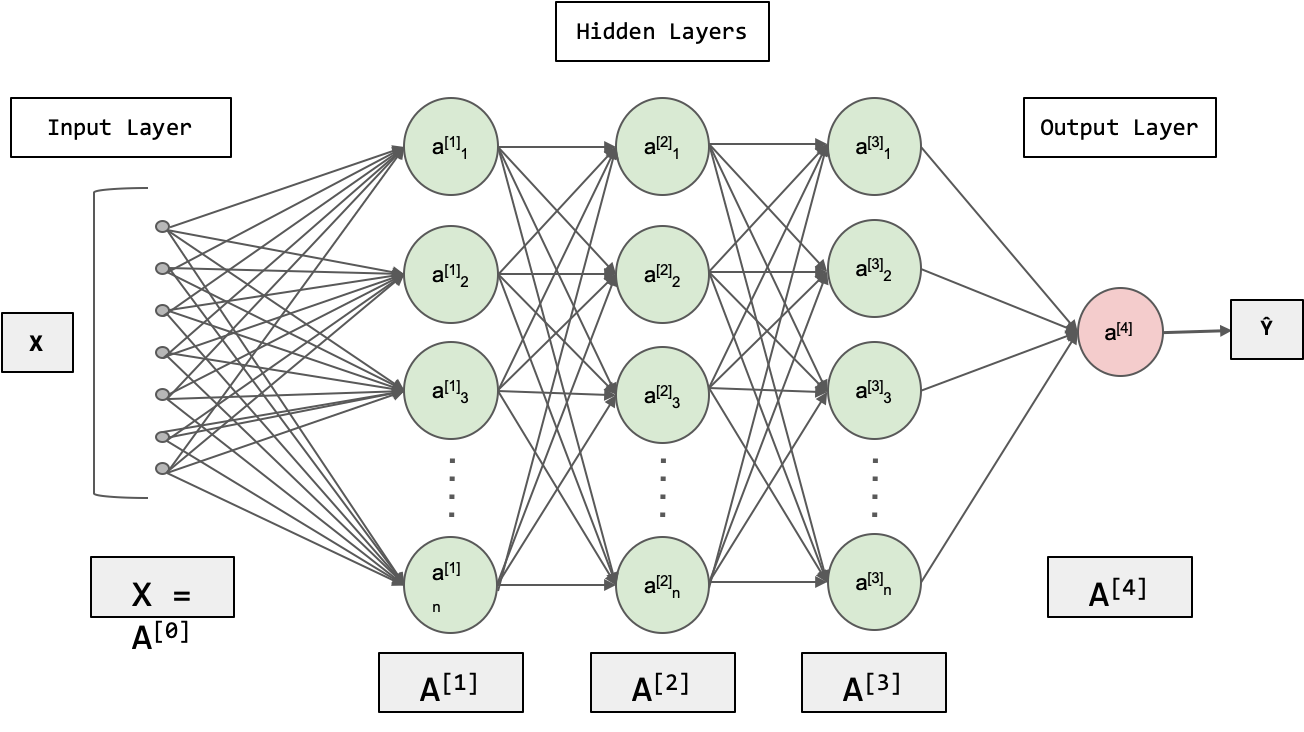
\includegraphics[width=0.4\textwidth]{pictures/MLP} %插入图片命令,格式为[配置]{图片路径}
    }
    \quad %空格
    \subfloat[]{
	\label{Fig:a2} % 子图2标签名
    	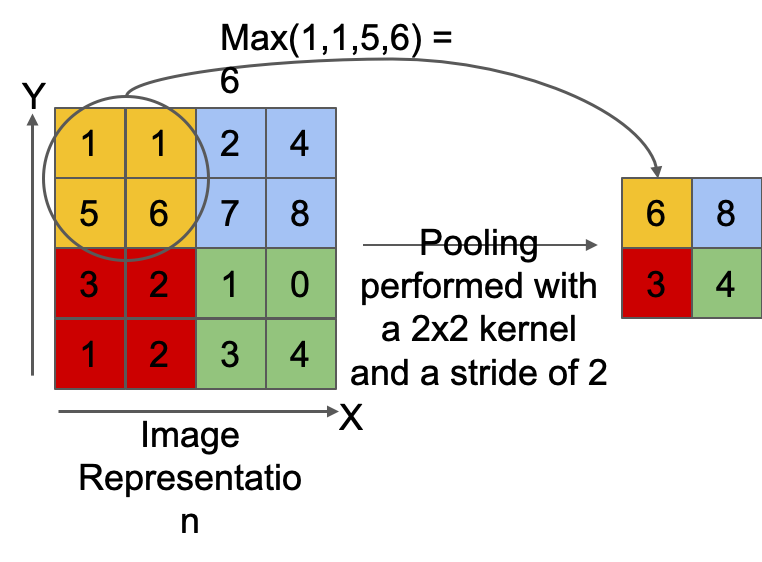
\includegraphics[width=0.4\textwidth]{pictures/maxpooling}
    }
    \caption{双图:\protect\subref{Fig:a1}图一,\protect\subref{Fig:a2}图二} %注意须使用\protect\subref{}进行标号引用
    \label{Fig:spamclass} % 整个组图的标签名
\end{figure}

\section{表格的插入}
基础表格如表2.1所示。
复杂表格设计可以使用https://www.tablesgenerator.com/,进行在线编辑然后复制粘贴即可。
\begin{xupttable}{混淆矩阵}{crowdwisdom2}
    \begin{tabular}{c|c|c}
        \hline \textbf{\ } & \textbf{实际假} & \textbf{实际真} \\
        \hline  \textbf{判定为假}& TP & FP \\
        \hline \textbf{判定为真} & FN & TN\\
        \hline
    \end{tabular}
\end{xupttable}

\section{伪代码的插入}
如Algorithm 1所示,提供了伪代码插入的参考。
\begin{algorithm}
	\begin{spacing}{1.3}
		\floatname{algorithm}{Algorithm}
		\caption{Reverse Auction-based Incentive} 
		\label{RAI}
		\renewcommand{\algorithmicrequire}{\textbf{Input:}}
		\renewcommand{\algorithmicensure}{\textbf{Output:}} 
			\begin{algorithmic}[1] 
				\Require 
				$v, b, R, U;$
				\Ensure $f, d;$
				\State 
				The MSP randomly divides the user set $V$ into two subsets $T$ and $Y$ , and then all vehicle users submit their respective quotations;
				\State 
				$Q_{T} \leftarrow OOA(T, R/2), Q_{Y} \leftarrow OOA(Y,R/2)$
				\State 
				$FRA\left(T, R/2, U Q_{Y}\right),FRA\left(Y, R/2, U Q_{T}\right)$    
				\State 
				Collecting the outputs of the two subsets to get $f$ and $d$; 
			    \State
		     	\Return{$\{f,d\}$}
			\end{algorithmic}
	\end{spacing}
\end{algorithm}

\chapter{参考文献的使用}
\section{校外文献检索}
人在校外,不在校内网范围,亦可使用中国知网、IEEE Xplore检索文献。(应该我不是最后一个知道的吧,不会吧,不会吧)
IEEE校外访问流程如图3.1-3.4所示。
\xuptfigure[width=0.8\textwidth]{pictures/IEEE1}{IEEE 访问流程一}{I1}
\xuptfigure[width=0.8\textwidth]{pictures/IEEE2}{IEEE 访问流程二}{I2}
\xuptfigure[width=0.8\textwidth]{pictures/IEEE3}{IEEE 访问流程三}{I3}
\xuptfigure[width=0.8\textwidth]{pictures/IEEE4}{IEEE 访问流程四}{I4}


中国知网校外访问流程如图3.5-3.8所示。
\xuptfigure[width=0.8\textwidth]{pictures/cnki1}{中国知网 访问流程一}{c1}
\xuptfigure[width=0.8\textwidth]{pictures/cnki2}{中国知网 访问流程二}{c2}
\xuptfigure[width=0.8\textwidth]{pictures/cnki3}{中国知网 访问流程三}{c3}
\xuptfigure[width=0.8\textwidth]{pictures/IEEE4}{中国知网 访问流程四}{c4}
\\
\\
\\
\\

\section{文献引用}
\citeauthor{lecun1995convolutional}指出对于数据的局部特征的关联性,全连接神经网络无法进行良好体现,而CNN则可以拥有局部感知、权重共享等特点\cite{lecun1995convolutional}。

通过Google Scholar检索文献并下载阅读,如图3.9所示,如需要引用则点击并复制BibTex,粘贴至ref.bib文件,在引用处通过$\setminus$ cite命令选择并完成引用。
\xuptfigure[width=1\textwidth]{pictures/cite}{Google Scholar参考文献}{cite}

\chapter{总结与展望}
本科毕业设计论文的书写,结构编排可以通过多阅读优秀硕士生毕业论文进行学习。

知网查重较贵,在初稿完成老师修改后,推荐使用其他第三方平台进行预查重(如果胆子比较大的话),比如:writepass(不是qia饭)。本人与西电,河海等部分同学使用过,若该查重低于20\%,校内查重一定通过。愿大家均可成功毕业,芜湖起飞。

\xuptfigure[width=0.3\textwidth]{pictures/fly}{芜湖起飞}{fly}

留两句很喜欢的词(源自:南京航空航天大学校歌)

效法羲和驭天马,志在长空牧群星。
越重关, 秉琴心剑胆, 御风行。

\xuptfigure[width=0.4\textwidth]{pictures/papershit}{Mypaper}{mypaper}

% Thanks to page
% 在main.cfg中编辑致谢内容
\clearpage\phantomsection\addcontentsline{toc}{chapter}{致\qquad{}谢}
\chapter*{致\qquad{}谢}
\normalsize\thankwords



% Reference
\clearpage\phantomsection\addcontentsline{toc}{chapter}{参考文献}
% XUPT网安院提高模板的参考文献格式为GB7714
\bibliographystyle{GB7714_XUPT}
% 文内所使用的所有参考文献加入至ref.bib
\refbodyfont{\bibliography{ref}}

% concluding remarks
%\clearpage\phantomsection\addcontentsline{toc}{chapter}{结束语}


%%%%%%%%%%%%%%%%%%%%%%%%%%%%%%%%%%%%%%%%%%%%%%%%%%%%%%%%%%%%%%%%%%
% 附录格式(无需调整)
\setcounter{figure}{0} 
\renewcommand{\thefigure}{~附-\arabic{figure}~}
\setcounter{equation}{0} 
\renewcommand{\theequation}{~附-\arabic{equation}~}
\setcounter{table}{0} 
\renewcommand{\thetable}{~附-\arabic{table}~}
\setcounter{lstlisting}{0} 
\makeatletter
  \renewcommand \thelstlisting
       {附-\@arabic\c@lstlisting}
\makeatother
%%%%%%%%%%%%%%%%%%%%%%%%%%%%%%%%%%%%%%%%%%%%%%%%%%%%%%%%%%%%%%%%%%


% Appendix
% 附录正文
\chapter*{附录A}
\phantomsection\addcontentsline{toc}{chapter}{附录}
\phantomsection


\end{document}
